\documentclass[a4paper]{CSMakotoTechnicalReport}

\addbibresource{sample.bib} % BibLaTeX bibliography file

\usepackage{amsmath}
\usepackage{tikz}
\usetikzlibrary{arrows,automata,positioning}

%----------------------------------------------------------------------------------------
%   REPORT INFORMATION
%----------------------------------------------------------------------------------------

\reporttitle{Procesador de MyJS: \textit{jsp}}

\reportsubtitle{Memoria del Grupo 59 (Primera Entrega)}

\reportauthors{Por Andrés Súnico (23M018)}

\reportdate{\today}

\leftheadercontent{Procesador de MyJS: \textit{jsp}}

%----------------------------------------------------------------------------------------

\begin{document}

%----------------------------------------------------------------------------------------
%   TITLE SECTION
%----------------------------------------------------------------------------------------

\thispagestyle{empty} % Suppress headers and footers on this page

\vspace*{0.08\textheight} % Vertical whitespace

{\large\raggedright\reportdate\par} % Report date

\vspace{0.01\textheight} % Vertical whitespace

{\fontsize{32pt}{34pt}\selectfont\raggedright\textbf{\reporttitle}\par} % Report title

\vspace{0.03\textheight} % Vertical whitespace

{\Large\raggedright\textit{\textbf{\reportsubtitle}}\par} % Subtitle

\vspace{0.06\textheight} % Vertical whitespace

{\large\raggedright\reportauthors\par} % Report authors, group or department

\vspace{0.36\textheight} % Vertical whitespace

%----------------------------------------------------------------------------------------

\begin{multicols}{2} % Begin two column mode

    %----------------------------------------------------------------------------------------
    %   TABLE OF CONTENTS
    %----------------------------------------------------------------------------------------

    \renewcommand{\contentsname}{Índice}
    \tableofcontents

    %----------------------------------------------------------------------------------------
    %   SECTIONS AND PARAGRAPHS
    %----------------------------------------------------------------------------------------

    \section{Introducción}

    El desarrollo del procesador \textit{jsp} se ha centrado en la experiencia del usuario (\textit{UX}), priorizando tres aspectos clave: una gestión de errores sólida y clara, una interfaz de línea de comandos (\textit{CLI}) intuitiva, y un rendimiento eficiente.

    Por ello, se ha elegido \textit{Rust} como el lenguaje de desarrollo. Ofrece una gestión de memoria eficiente, además de integrar \textit{clap}, una de las mejores librerías para desarollar aplicaciones \textit{CLI}.

    Gracias al uso del patrón de \textit{inyección de dependencias} en todo el proyecto, el código fuente es altamente extensible y modular.

    \section{Información Adicional}

    El código fuente del procesador se puede encontrar en \href{https://www.github.com/suuniqo}{github.com/suuniqo}, así como los tests y las dependencias del proyecto.

    \section{Opciones de la práctica}

    Además de las opciones comunes a todos los grupos, se han implementado las opciones:

    \subsection{Específicas del grupo}

    \begin{itemize}
        \item Comentarios de bloque (/* */)
        \item Cadenas con comillas dobles (" ")
        \item Sentencia repetitiva do-while
        \item Asignación con \textit{y} lógico (\textit{\&=})
        \item Análisis Sintáctico Ascendente
    \end{itemize}

    \subsection{Adicionales}

    Para que el procesador esté más completo, se han implementado adicionalmente todos los operadores lógicos, aritméticos, relacionales y unarios, así como los \textit{tokens} booleanos \textit{true} y \textit{false}.

    Además se ha escogido implementar el tratamiento de secuencias de escape (\textit{\textbackslash n} y \textit{\textbackslash t}).


    \section{Diseño del Lexer}
    
    El Analizador Léxico o \textit{Lexer} es uno de los 3 módulos principales del procesador.

    Al ser la primera capa de procesamiento, es el encargado de manejar el fichero fuente y convertirlo en una lista de \textit{tokens} para el Analizador Sintáctico.

    \subsection{Tokens}

    Con el fin de lograr un procesamiento eficiente, tanto en memoria como en complejidad, se han minimizado el número de \textit{tokens} con atributos.

    De este modo sólo 4 de un total de 41 \textit{tokens} van a utilizar un atributo.

    Cabe notar, además, que se ha decidido no hacer uso del \textit{token} fin de fichero (\textit{EOF}). Esto es porque el \textit{Lexer} se ha implementado como un iterador de \textit{tokens}, de modo que el final del flujo se detecta naturalmente cuando se consume el iterador.

    \renewcommand{\arraystretch}{1.2}
    \begin{table}[H]
        \caption{Listado de \textit{tokens}}
        \begin{tabular}{L{0.35\linewidth} L{0.31\linewidth} L{0.17\linewidth}}
            \toprule
            \textbf{Elemento} & \textbf{Código} & \textbf{Atributo} \\
            \midrule
            boolean & Bool & - \\
            do & Do & - \\
            float & Float & - \\
            function & Func & - \\
            if & If & - \\
            int & Int & - \\
            let & Let & - \\
            read & Read & - \\
            return & Ret & - \\
            string & Str & - \\
            void & Void & - \\
            while & While & - \\
            write & Write & - \\
            constante real & FloatLit & Número \\
            constante entera & IntLit & Número \\
            Cadena & StrLit & Cadena \\
            Identificador & Id & Posición \\
            \&= & AndAssign & - \\
            = & Assign & - \\
            , & Comma & - \\
            ; & Semi & - \\
            ( & LParen & - \\
            ) & RParen & - \\
            \{ & LBrack & - \\
            \} & RBrack & - \\
            Suma (+) & Sum & - \\
            Por (*) & Mul & - \\
            Resta (-) & Sub & - \\
            División (/) & Div & - \\
            Módulo (\%) & Mod & - \\
            Y lógico (\&\&) & And & - \\
            O lógico (||) & Or & - \\
            Negación (!) & Not & - \\
            Menor (<) & Lt & - \\
            Menor o igual (<=) & Le & - \\
            Mayor (>) & Gt & - \\
            Mayor o igual (>=) & Ge & - \\
            Relacionales: Distinto (!=) & Ne & - \\
            Igual (==) & Eq & - \\
            Menos Unario (-) & Sub & - \\
            Más Unario (+) & Sum & - \\
            false & False & - \\
            true & True & - \\
            \bottomrule
        \end{tabular}
        \label{tab:example}
    \end{table}

    \subsection{Errores}

    El diseño de los errores y del gestor está orientado a la \textit{UX}. Cada tipo de error consta de un mensaje diferente y de una severidad, distinguiéndose \textit{errors} de \textit{warnings} (que no impedirían la compilación del programa).

    El procesador genera mensajes claros con número de línea y columna, muestra la línea afectada y subraya en color (que depende de la severidad) la parte errónea.

    El \textit{Lexer} sólo genera un warning, \textit{Invalid Escape Sequence}. Como se muestra en \hyperref[subsec:acciones-semanticas]{Acciones Semánticas}, al detectar una secuencia de escape inválida no se descartara el \textit{token} cadena, sino que se conserva literalmente (por ejemplo, la secuencia \textit{\textbackslash q}, se sustituye por esos dos mismos caracteres).

    \renewcommand{\arraystretch}{1.5}
    \begin{table}[H]
        \caption{Listado de errores del \textit{Lexer}}
        \begin{tabular}{L{0.63\linewidth} L{0.20\linewidth}}
            \toprule
            \textbf{Error} & \textbf{Severidad} \\
            \midrule
            Carácter inválido & \textit{error} \\
            Comentario inacabado & \textit{error} \\
            Cadena inacabada & error \\
            Overflow de Cadena & \textit{error} \\
            Overflow de Entero & \textit{error} \\
            Overflow de Real & \textit{error} \\
            Formato de Real Inválido & \textit{error} \\
            Secuencia de Escape Inválida & \textit{warning} \\
            \bottomrule
        \end{tabular}
        \label{tab:example}
    \end{table}
\end{multicols}

    \subsection{Gramática}

    Se define la gramática del \textit{Lexer} como $G = (T, N, S, P)$, dónde:
    \begin{flalign*}
        T &= \{ \textnormal{Todo carácter \textit{ASCII}} \} \cup \{\textit{EOF}\} && \\
        N &= \{A, B, C, D, E, F, G, H, I, J, K, L, M\} &&
    \end{flalign*}
     $P$ se compone de las reglas:
    \begin{flalign*}
        S &\to \textnormal{del}S \;\mid\; , \;\mid\; ; \;\mid\; ( \;\mid\; ) \;\mid\; \{ \;\mid\; \} \;\mid\; + \;\mid\; * \;\mid\; \% \;\mid\; =A \;\mid\; !B \;\mid\; <C \;\mid\; >D \;\mid\; \&E \;\mid\; |F \;\mid\; dG \;\mid\; "H \;\mid\; c_1I \;\mid\; /J \;\mid\; \textit{EOF} && \\
        A &\to \; = \;\mid\; \lambda && \\
        B &\to \; = \;\mid\; \lambda && \\
        C &\to \; = \;\mid\; \lambda && \\
        D &\to \; = \;\mid\; \lambda && \\
        E &\to \; = \;\mid\; \lambda && \\
        F &\to \; | && \\
        G &\to dG \;\mid\; .K \;\mid\; \lambda && \\
        K &\to dK \;\mid\; \lambda && \\
        H &\to c_2H \;\mid\; \backslash L \;\mid\; " && \\
        L &\to \textnormal{n}H \;\mid\; \textnormal{t}H && \\
        I &\to c_3I \;\mid\; \lambda && \\
        J &\to *M \;\mid\; \lambda && \\
        M &\to c_4M \;\mid\; *N && \\
        N &\to c_5M \;\mid\; *N \;\mid\; /S &&
    \end{flalign*}
    Y se definen:
    \begin{flalign*}
        d &:= \{0, 1, \dots, 9\} && \\
        l &:= \{\textnormal{a}, \textnormal{b}, \dots, \textnormal{z}, \textnormal{A}, \textnormal{B}, \dots, \textnormal{Z}\} && \\
        c_1 &:= l \cup \{\_\} && \\
        c_2 &:= T \setminus (\{\backslash, ", \textit{EOF}\} \cup \{\textnormal{Todos los caracteres \textit{ASCII} no gráficos (Es decir, con código menor que 32)\}}) && \\
        c_3 &:= c_1 \cup d && \\
        c_4 &:= T \setminus \{*, \textit{EOF}\} && \\
        c_5 &:= T \setminus \{*, /, \textit{EOF}\} && \\
    \end{flalign*}


    \subsection{Autómata}

    A continuación se muestra el autómata finito determinista que reconoce el lenguaje generado por la gramática $G$. Una transición "o.c." ocurre al leer un carácter que no corresponda a otra transición del estado.

    \begin{figure}[ht]
        \centering
        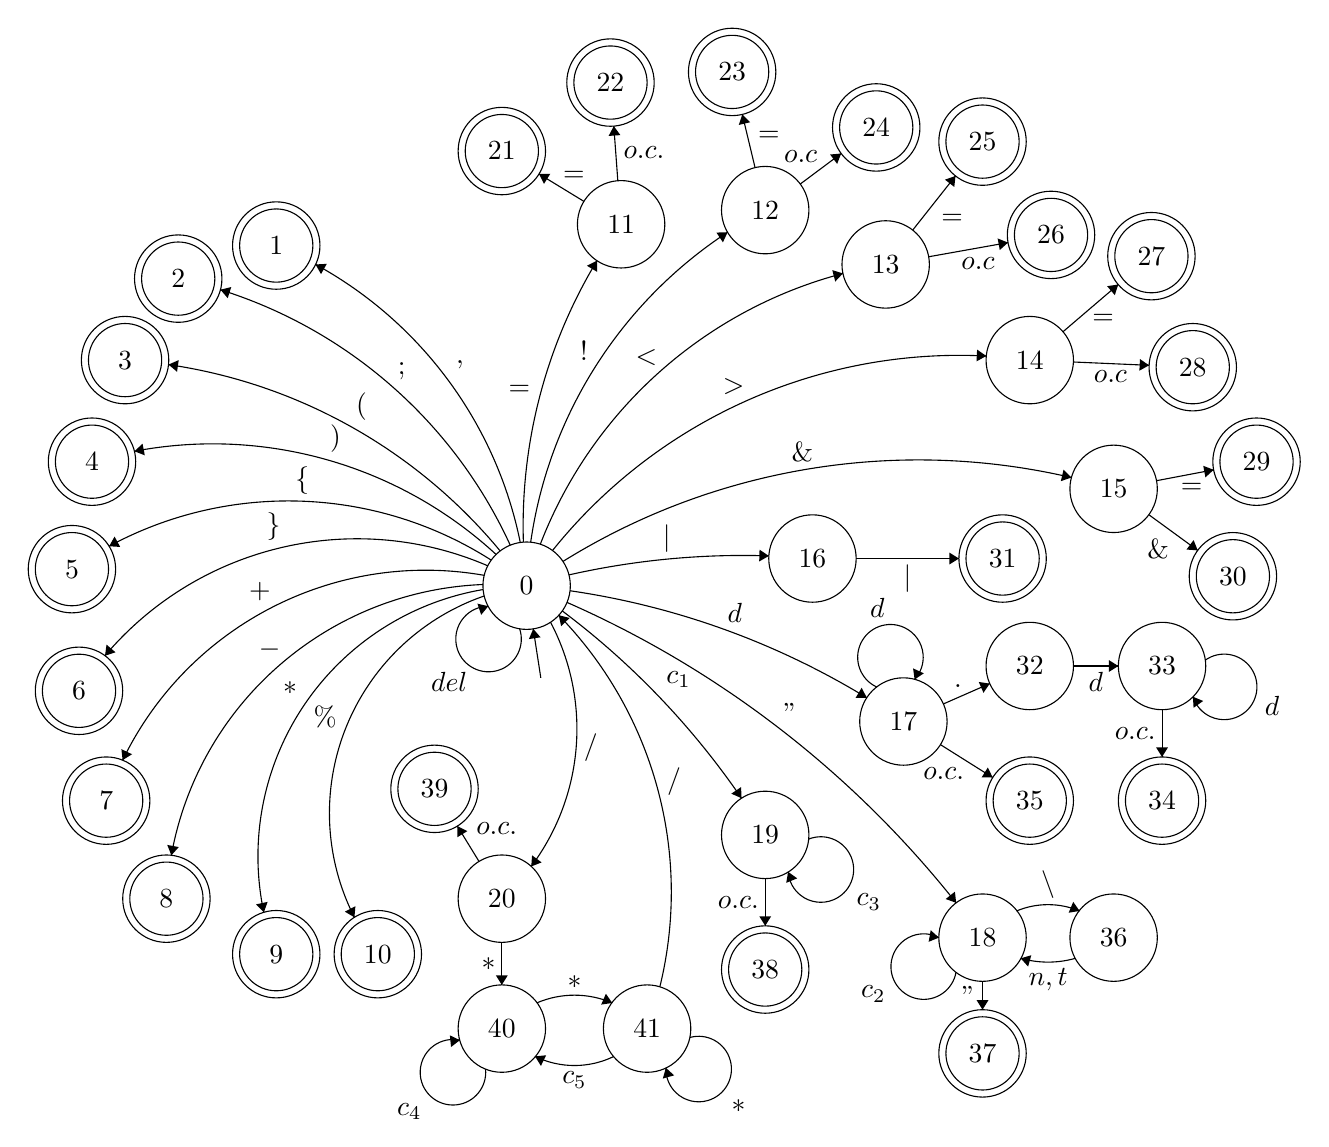
\begin{tikzpicture}[scale=0.15]
            \tikzstyle{every node}+=[inner sep=0pt]
            \draw [black] (42.4,-47.4) circle (3.7);
            \draw (42.4,-47.4) node {$0$};
            \draw [black] (21.2,-18.6) circle (3.7);
            \draw (21.2,-18.6) node {$1$};
            \draw [black] (21.2,-18.6) circle (3.1);
            \draw [black] (12.9,-21.4) circle (3.7);
            \draw (12.9,-21.4) node {$2$};
            \draw [black] (12.9,-21.4) circle (3.1);
            \draw [black] (8.4,-28.3) circle (3.7);
            \draw (8.4,-28.3) node {$3$};
            \draw [black] (8.4,-28.3) circle (3.1);
            \draw [black] (5.6,-36.9) circle (3.7);
            \draw (5.6,-36.9) node {$4$};
            \draw [black] (5.6,-36.9) circle (3.1);
            \draw [black] (3.9,-46) circle (3.7);
            \draw (3.9,-46) node {$5$};
            \draw [black] (3.9,-46) circle (3.1);
            \draw [black] (4.5,-56.3) circle (3.7);
            \draw (4.5,-56.3) node {$6$};
            \draw [black] (4.5,-56.3) circle (3.1);
            \draw [black] (6.8,-65.6) circle (3.7);
            \draw (6.8,-65.6) node {$7$};
            \draw [black] (6.8,-65.6) circle (3.1);
            \draw [black] (11.9,-73.9) circle (3.7);
            \draw (11.9,-73.9) node {$8$};
            \draw [black] (11.9,-73.9) circle (3.1);
            \draw [black] (21.2,-78.6) circle (3.7);
            \draw (21.2,-78.6) node {$9$};
            \draw [black] (21.2,-78.6) circle (3.1);
            \draw [black] (29.8,-78.6) circle (3.7);
            \draw (29.8,-78.6) node {$10$};
            \draw [black] (29.8,-78.6) circle (3.1);
            \draw [black] (50.4,-16.8) circle (3.7);
            \draw (50.4,-16.8) node {$11$};
            \draw [black] (62.6,-15.6) circle (3.7);
            \draw (62.6,-15.6) node {$12$};
            \draw [black] (72.8,-20.2) circle (3.7);
            \draw (72.8,-20.2) node {$13$};
            \draw [black] (85,-28.3) circle (3.7);
            \draw (85,-28.3) node {$14$};
            \draw [black] (92.1,-39.2) circle (3.7);
            \draw (92.1,-39.2) node {$15$};
            \draw [black] (66.6,-45.1) circle (3.7);
            \draw (66.6,-45.1) node {$16$};
            \draw [black] (74.3,-58.9) circle (3.7);
            \draw (74.3,-58.9) node {$17$};
            \draw [black] (81,-77.2) circle (3.7);
            \draw (81,-77.2) node {$18$};
            \draw [black] (62.6,-68.5) circle (3.7);
            \draw (62.6,-68.5) node {$19$};
            \draw [black] (40.3,-73.9) circle (3.7);
            \draw (40.3,-73.9) node {$20$};
            \draw [black] (40.3,-10.6) circle (3.7);
            \draw (40.3,-10.6) node {$21$};
            \draw [black] (40.3,-10.6) circle (3.1);
            \draw [black] (49.5,-4.8) circle (3.7);
            \draw (49.5,-4.8) node {$22$};
            \draw [black] (49.5,-4.8) circle (3.1);
            \draw [black] (59.8,-3.9) circle (3.7);
            \draw (59.8,-3.9) node {$23$};
            \draw [black] (59.8,-3.9) circle (3.1);
            \draw [black] (72,-8.6) circle (3.7);
            \draw (72,-8.6) node {$24$};
            \draw [black] (72,-8.6) circle (3.1);
            \draw [black] (81,-9.8) circle (3.7);
            \draw (81,-9.8) node {$25$};
            \draw [black] (81,-9.8) circle (3.1);
            \draw [black] (86.8,-17.7) circle (3.7);
            \draw (86.8,-17.7) node {$26$};
            \draw [black] (86.8,-17.7) circle (3.1);
            \draw [black] (95.3,-19.5) circle (3.7);
            \draw (95.3,-19.5) node {$27$};
            \draw [black] (95.3,-19.5) circle (3.1);
            \draw [black] (98.8,-28.9) circle (3.7);
            \draw (98.8,-28.9) node {$28$};
            \draw [black] (98.8,-28.9) circle (3.1);
            \draw [black] (104.2,-36.9) circle (3.7);
            \draw (104.2,-36.9) node {$29$};
            \draw [black] (104.2,-36.9) circle (3.1);
            \draw [black] (102.2,-46.6) circle (3.7);
            \draw (102.2,-46.6) node {$30$};
            \draw [black] (102.2,-46.6) circle (3.1);
            \draw [black] (82.7,-45.1) circle (3.7);
            \draw (82.7,-45.1) node {$31$};
            \draw [black] (82.7,-45.1) circle (3.1);
            \draw [black] (85,-54.2) circle (3.7);
            \draw (85,-54.2) node {$32$};
            \draw [black] (85,-65.6) circle (3.7);
            \draw (85,-65.6) node {$35$};
            \draw [black] (85,-65.6) circle (3.1);
            \draw [black] (96.2,-54.2) circle (3.7);
            \draw (96.2,-54.2) node {$33$};
            \draw [black] (96.2,-65.6) circle (3.7);
            \draw (96.2,-65.6) node {$34$};
            \draw [black] (96.2,-65.6) circle (3.1);
            \draw [black] (92.1,-77.2) circle (3.7);
            \draw (92.1,-77.2) node {$36$};
            \draw [black] (81,-87) circle (3.7);
            \draw (81,-87) node {$37$};
            \draw [black] (81,-87) circle (3.1);
            \draw [black] (62.6,-79.9) circle (3.7);
            \draw (62.6,-79.9) node {$38$};
            \draw [black] (62.6,-79.9) circle (3.1);
            \draw [black] (34.6,-64.6) circle (3.7);
            \draw (34.6,-64.6) node {$39$};
            \draw [black] (34.6,-64.6) circle (3.1);
            \draw [black] (40.3,-84.9) circle (3.7);
            \draw (40.3,-84.9) node {$40$};
            \draw [black] (52.6,-84.9) circle (3.7);
            \draw (52.6,-84.9) node {$41$};
            \draw [black] (41.806,-51.037) arc (18.45967:-269.54033:2.775);
            \draw (35.84,-54.67) node [below,align=center] {$del$};
            \fill [black] (39.15,-49.14) -- (38.23,-48.92) -- (38.55,-49.87);
            \draw [black] (43.6,-55.2) -- (42.96,-51.06);
            \fill [black] (42.96,-51.06) -- (42.59,-51.92) -- (43.58,-51.77);
            \draw [black] (24.534,-20.201) arc (61.28524:11.42915:34.675);
            \fill [black] (24.53,-20.2) -- (24.99,-21.02) -- (25.48,-20.15);
            \draw (36.38,-28.67) node [right,align=center] {$,$};
            \draw [black] (16.476,-22.345) arc (72.57177:24.64517:40.265);
            \fill [black] (16.48,-22.34) -- (17.09,-23.06) -- (17.39,-22.11);
            \draw (31.83,-30.06) node [above,align=center] {$;$};
            \draw [black] (12.079,-28.682) arc (81.70676:39.64176:44.871);
            \fill [black] (12.08,-28.68) -- (12.8,-29.29) -- (12.94,-28.3);
            \draw (28.41,-33.46) node [above,align=center] {$($};
            \draw [black] (9.192,-36.018) arc (100.80772:47.34262:35.397);
            \fill [black] (9.19,-36.02) -- (10.07,-36.36) -- (9.88,-35.38);
            \draw (26.21,-36.2) node [above,align=center] {$)$};
            \draw [black] (7.047,-44.058) arc (118.36416:57.47071:31.947);
            \fill [black] (7.05,-44.06) -- (7.99,-44.12) -- (7.51,-43.24);
            \draw (23.41,-39.71) node [above,align=center] {$\{$};
            \draw [black] (6.696,-53.326) arc (139.76528:66.6652:27.954);
            \fill [black] (6.7,-53.33) -- (7.59,-53.04) -- (6.83,-52.39);
            \draw (20.98,-43.59) node [above,align=center] {$\}$};
            \draw [black] (8.193,-62.175) arc (154.15624:79.99927:28.515);
            \fill [black] (8.19,-62.17) -- (8.99,-61.67) -- (8.09,-61.24);
            \draw (19.82,-48.71) node [above,align=center] {$+$};
            \draw [black] (12.317,-70.226) arc (169.72878:92.24287:27.928);
            \fill [black] (12.32,-70.23) -- (12.95,-69.53) -- (11.97,-69.35);
            \draw (20.64,-53.63) node [above,align=center] {$-$};
            \draw [black] (20.146,-75.057) arc (-168.05628:-260.33493:22.916);
            \fill [black] (20.15,-75.06) -- (20.47,-74.17) -- (19.49,-74.38);
            \draw (23.01,-56.09) node [left,align=center] {$*$};
            \draw [black] (27.819,-75.482) arc (-153.02437:-250.95789:19.453);
            \fill [black] (27.82,-75.48) -- (27.9,-74.54) -- (27.01,-75);
            \draw (26.37,-58.48) node [left,align=center] {$\%$};
            \draw [black] (42.125,-43.711) arc (-178.18269:-211.12003:43.44);
            \fill [black] (48.36,-19.88) -- (47.51,-20.31) -- (48.37,-20.83);
            \draw (42.75,-30.85) node [left,align=center] {$=$};
            \draw [black] (42.743,-43.717) arc (171.87908:123.27185:37.769);
            \fill [black] (59.41,-17.48) -- (58.47,-17.5) -- (59.02,-18.33);
            \draw (47.63,-27.5) node [left,align=center] {$!$};
            \draw [black] (43.559,-43.888) arc (158.92154:104.7188:37.734);
            \fill [black] (69.18,-20.96) -- (68.28,-20.68) -- (68.53,-21.65);
            \draw (52.53,-28.85) node [above,align=center] {$<$};
            \draw [black] (44.592,-44.421) arc (141.25458:87.04423:44.167);
            \fill [black] (81.32,-27.95) -- (80.54,-27.41) -- (80.49,-28.41);
            \draw (59.93,-31.25) node [above,align=center] {$>$};
            \draw [black] (45.476,-45.345) arc (121.87872:76.85893:56.985);
            \fill [black] (88.53,-38.24) -- (87.86,-37.57) -- (87.63,-38.55);
            \draw (65.74,-36.89) node [above,align=center] {$\&$};
            \draw [black] (45.985,-46.485) arc (102.73111:88.12721:66.873);
            \fill [black] (62.91,-44.88) -- (62.12,-44.35) -- (62.09,-45.35);
            \draw (54.27,-44.59) node [above,align=center] {$|$};
            \draw [black] (46.075,-47.829) arc (81.74377:58.6076:66.585);
            \fill [black] (71.2,-56.89) -- (70.77,-56.04) -- (70.25,-56.9);
            \draw (60.02,-50.56) node [above,align=center] {$d$};
            \draw [black] (45.818,-48.815) arc (66.278:38.38423:86.347);
            \fill [black] (78.77,-74.25) -- (78.66,-73.31) -- (77.88,-73.93);
            \draw (64.76,-59.02) node [above,align=center] {$"$};
            \draw [black] (45.419,-49.539) arc (53.10827:34.39498:67.492);
            \fill [black] (60.59,-65.39) -- (60.56,-64.45) -- (59.73,-65.01);
            \draw (54.18,-55.37) node [right,align=center] {$c_1$};
            \draw [black] (44.424,-50.491) arc (27.75739:-36.81929:19.414);
            \fill [black] (42.79,-71.17) -- (43.67,-70.83) -- (42.86,-70.23);
            \draw (47.21,-61.12) node [right,align=center] {$/$};
            \draw [black] (47.25,-14.86) -- (43.45,-12.54);
            \fill [black] (43.45,-12.54) -- (43.87,-13.38) -- (44.4,-12.53);
            \draw (46.41,-13.2) node [above,align=center] {$=$};
            \draw [black] (50.12,-13.11) -- (49.78,-8.49);
            \fill [black] (49.78,-8.49) -- (49.34,-9.32) -- (50.34,-9.25);
            \draw (50.56,-10.75) node [right,align=center] {$o.c.$};
            \draw [black] (61.74,-12) -- (60.66,-7.5);
            \fill [black] (60.66,-7.5) -- (60.36,-8.39) -- (61.33,-8.16);
            \draw (61.96,-9.32) node [right,align=center] {$=$};
            \draw [black] (65.57,-13.39) -- (69.03,-10.81);
            \fill [black] (69.03,-10.81) -- (68.09,-10.89) -- (68.69,-11.69);
            \draw (65.6,-11.6) node [above,align=center] {$o.c$};
            \draw [black] (75.09,-17.29) -- (78.71,-12.71);
            \fill [black] (78.71,-12.71) -- (77.82,-13.02) -- (78.61,-13.64);
            \draw (77.47,-16.42) node [right,align=center] {$=$};
            \draw [black] (76.44,-19.55) -- (83.16,-18.35);
            \fill [black] (83.16,-18.35) -- (82.28,-18) -- (82.46,-18.98);
            \draw (80.62,-19.61) node [below,align=center] {$o.c$};
            \draw [black] (87.81,-25.9) -- (92.49,-21.9);
            \fill [black] (92.49,-21.9) -- (91.55,-22.04) -- (92.2,-22.8);
            \draw (91.22,-24.39) node [below,align=center] {$=$};
            \draw [black] (88.7,-28.46) -- (95.1,-28.74);
            \fill [black] (95.1,-28.74) -- (94.33,-28.21) -- (94.28,-29.2);
            \draw (91.83,-29.17) node [below,align=center] {$o.c$};
            \draw [black] (95.73,-38.51) -- (100.57,-37.59);
            \fill [black] (100.57,-37.59) -- (99.69,-37.25) -- (99.87,-38.23);
            \draw (98.71,-38.65) node [below,align=center] {$=$};
            \draw [black] (95.08,-41.39) -- (99.22,-44.41);
            \fill [black] (99.22,-44.41) -- (98.87,-43.54) -- (98.27,-44.34);
            \draw (95.87,-43.4) node [below,align=center] {$\&$};
            \draw [black] (70.3,-45.1) -- (79,-45.1);
            \fill [black] (79,-45.1) -- (78.2,-44.6) -- (78.2,-45.6);
            \draw (74.65,-45.6) node [below,align=center] {$|$};
            \draw [black] (72.048,-55.982) arc (245.39558:-42.60442:2.775);
            \draw (72.09,-50.15) node [above,align=center] {$d$};
            \fill [black] (75.25,-55.34) -- (76.03,-54.82) -- (75.12,-54.4);
            \draw [black] (77.69,-57.41) -- (81.61,-55.69);
            \fill [black] (81.61,-55.69) -- (80.68,-55.55) -- (81.08,-56.47);
            \draw (78.92,-56.04) node [above,align=center] {$.$};
            \draw [black] (77.44,-60.86) -- (81.86,-63.64);
            \fill [black] (81.86,-63.64) -- (81.45,-62.79) -- (80.92,-63.64);
            \draw (77.71,-62.75) node [below,align=center] {$o.c.$};
            \draw [black] (88.7,-54.2) -- (92.5,-54.2);
            \fill [black] (92.5,-54.2) -- (91.7,-53.7) -- (91.7,-54.7);
            \draw (90.6,-54.7) node [below,align=center] {$d$};
            \draw [black] (99.852,-53.707) arc (125.41506:-162.58494:2.775);
            \draw (104.86,-57.56) node [right,align=center] {$d$};
            \fill [black] (98.81,-56.8) -- (98.87,-57.74) -- (99.68,-57.16);
            \draw [black] (96.2,-57.9) -- (96.2,-61.9);
            \fill [black] (96.2,-61.9) -- (96.7,-61.1) -- (95.7,-61.1);
            \draw (95.7,-59.9) node [left,align=center] {$o.c.$};
            \draw [black] (78.755,-80.123) arc (-9.80292:-297.80292:2.775);
            \draw (72.83,-81.97) node [left,align=center] {$c_2$};
            \fill [black] (77.31,-77.2) -- (76.61,-76.57) -- (76.44,-77.55);
            \draw [black] (83.876,-74.943) arc (112.76955:67.23045:6.908);
            \fill [black] (89.22,-74.94) -- (88.68,-74.17) -- (88.29,-75.09);
            \draw (86.55,-73.91) node [above,align=center] {$\backslash$};
            \draw [black] (88.872,-78.947) arc (-74.09162:-105.90838:8.471);
            \fill [black] (84.23,-78.95) -- (84.86,-79.65) -- (85.13,-78.69);
            \draw (86.55,-79.77) node [below,align=center] {$n,t$};
            \draw [black] (81,-80.9) -- (81,-83.3);
            \fill [black] (81,-83.3) -- (81.5,-82.5) -- (80.5,-82.5);
            \draw (80.5,-82.1) node [left,align=center] {$"$};
            \draw [black] (66.268,-68.861) arc (112.11578:-175.88422:2.775);
            \draw (70.3,-74.19) node [right,align=center] {$c_3$};
            \fill [black] (64.54,-71.63) -- (64.38,-72.56) -- (65.31,-72.18);
            \draw [black] (62.6,-72.2) -- (62.6,-76.2);
            \fill [black] (62.6,-76.2) -- (63.1,-75.4) -- (62.1,-75.4);
            \draw (62.1,-74.2) node [left,align=center] {$o.c.$};
            \draw [black] (38.37,-70.75) -- (36.53,-67.75);
            \fill [black] (36.53,-67.75) -- (36.53,-68.7) -- (37.38,-68.18);
            \draw (38.09,-67.97) node [right,align=center] {$o.c.$};
            \draw [black] (40.3,-77.6) -- (40.3,-81.2);
            \fill [black] (40.3,-81.2) -- (40.8,-80.4) -- (39.8,-80.4);
            \draw (39.8,-79.4) node [left,align=center] {$*$};
            \draw [black] (38.921,-88.318) arc (5.7603:-282.2397:2.775);
            \draw (33.55,-91.9) node [left,align=center] {$c_4$};
            \fill [black] (36.75,-85.88) -- (35.9,-85.47) -- (36,-86.46);
            \draw [black] (43.255,-82.727) arc (113.24615:66.75385:8.096);
            \fill [black] (49.65,-82.73) -- (49.11,-81.95) -- (48.71,-82.87);
            \draw (46.45,-81.57) node [above,align=center] {$*$};
            \draw [black] (49.793,-87.254) arc (-63.93898:-116.06102:7.61);
            \fill [black] (43.11,-87.25) -- (43.61,-88.06) -- (44.05,-87.16);
            \draw (46.45,-88.53) node [below,align=center] {$c_5$};
            \draw [black] (56.207,-85.657) arc (105.87903:-182.12097:2.775);
            \draw (59.72,-91.45) node [right,align=center] {$*$};
            \fill [black] (54.19,-88.22) -- (53.93,-89.13) -- (54.89,-88.86);
            \draw [black] (45.122,-49.904) arc (44.2371:-13.80445:33.602);
            \fill [black] (45.12,-49.9) -- (45.32,-50.83) -- (46.04,-50.13);
            \draw (54.24,-64) node [right,align=center] {$/$};
        \end{tikzpicture}
        \vspace{0.02\textheight}
        \caption{Autómata que reconoce el lenguaje $L(G)$}
        \label{fig:automaton}
    \end{figure}

    \subsection{Acciones Semánticas}
    \label{subsec:acciones-semanticas}

    \begin{lstlisting}
        {
            "city": [
            {
                "id": 1,
                "name": "Toronto",
                "country": "Canada",
                "population": 6200000
            },
            {
                "id": 2,
                "name": "New York",
                "country": "United States of America",
                "population": 8800000
            }
            ]
        }
    \end{lstlisting}

    \section{Diseño de la Tabla de Símbolos}
    \subsection{Estructura y Organización}

    \section{Diseño del Parser}
    \section{Diseño del Semanter}
    \section{Gestor de Errores}

%----------------------------------------------------------------------------------------
%   APPENDICES
%----------------------------------------------------------------------------------------

\newpage

\section*{Appendices}

\begin{appendices}

    \section{Casos de Prueba}

    Lorem ipsum dolor sit amet, consectetur adipiscing elit. Aliquam auctor mi risus, quis tempor libero hendrerit at. Duis hendrerit placerat quam et semper. Nam ultricies metus vehicula arcu viverra, vel ullamcorper justo elementum. Pellentesque vel mi ac lectus cursus posuere et nec ex. Fusce quis mauris egestas lacus commodo venenatis. Ut at arcu lectus. Donec et urna nunc. Morbi eu nisl cursus sapien eleifend tincidunt quis quis est. Donec ut orci ex. Praesent ligula enim, ullamcorper non lorem a, ultrices volutpat dolor. Nullam at imperdiet urna. Pellentesque nec velit eget euismod pretium.

\end{appendices}

%----------------------------------------------------------------------------------------

\end{document}

